\section{Zielsetzung}
\label{sec:Zielsetzung}

Ziel des Versuchs ist die Bestimmung der Materialien von neun Würfeln
anhand ihrer Absorptionskoeffizienten.
Diese befinden sich in einem Aluminiumgehäuse in drei Schichten von
jeweils drei mal drei Würfeln.

\section{Theorie}
\label{sec:Theorie}

\subsection{Gamma-Spektrum}
\label{sec:GammaSpektrum}

Wird die Intensität von Strahlung nach Durchlauf einer Probe gegen die Wellenlänge
aufgetragen, ergibt sich ein typischer Verlauf, welcher aus den unterschiedlichen
Wechselwirkungen der Strahlung im Material resultiert.
Dieser Verlauf wird für Photonen beziehungsweise $\gamma$-Strahlung
auch \enquote{$\gamma$-Spektrum} genannt.
Für große Wellenlängen dominiert der Comptoneffekt,
welcher zu einer kontinierlichen Absorptionslinie
bis zur sogenannten \enquote{Comptonkante} führt.
Diese Comptonkante befindet sich bei der Wellenlänge,
bei welcher ein einfallendes Photon einen maximalen
Energieübertrag an das Elektron leistet.
Deshalb sinkt die Intensität der die Probe durchlaufenden Strahlung
bei dieser Wellenlänge abrupt.
Bei etwas höheren Wellenlängen ist ein Peak messbar,
welche auf dem Photoeffekt beruht, der sogenannte \enquote{Photopeak}.
Bei noch kleineren Wellenlängen steigt die Intensität wieder an,
da der Effekt der \enquote{Paarerzeugung} auftritt.
Hierbei bildet sich aus der Photonenenergie ein Teilchen-Antiteilchen-Paar.
Dazu muss jedoch die Energie des Photons mindestens der Ruheenergie
des Teilchen-Antiteilchen-Paares entsprechen.

\begin{figure}
  \centering
  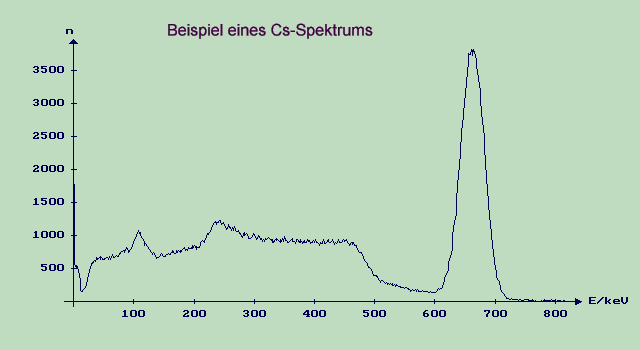
\includegraphics[height=8.0cm]{content/Energiespektrum.jpg}
  \caption{Beispiel eines $\gamma$-Spektrums für \ce{^137Cs} \cite{hans}.
  Aufgetragen ist die Anzahl an Ereignissen in Abhängigkeit der Energie.}
  \label{fig:spektrum}
\end{figure}

Ein Beispiel eines solchen Absorptionsspektrums ist in Abbildung \ref{fig:spektrum}
dargestellt. Hier ist die Anzahl an gemessenen Ereignissen für ein
festes Zeitintervall gegen die Photonenenergie aufgetragen.
Für kleine Energien ist die kontinuierliche Absorptionslinie des Comptoneffekts
und die Comptonkante bei ungefähr \SI{480}{\kilo\electronvolt} erkennbar
und bei grob \SI{680}{\kilo\electronvolt}
befindet sich der Photopeak. Die Paarerzeugung ist nicht abgebildet,
da sie erst bei höheren Energien auftritt.


\subsection{Tomographie}
\label{sec:Tomographie}

% Tomographie
Tomographie ist ein Verfahren, bei welchem aus verschiedenen
Querschnittsbildern ein Objekt räumlich abgebildet wird.
Es wird unter anderem bei der Untersuchung von Menschen auf Tumorgewebe eingesetzt,
da sich auch kleine Dichteunterschiede der Organe deutlich erkennen lassen \cite{paradisi}.
In diesem Versuch wird dazu $\gamma$-Strahlung verwendet.
Trifft $\gamma$-Strahlung auf Materie, verringert sich die Intensität $N$
nach der Strecke $r$ von $N_0$ auf
\begin{equation*}
  N\left(r\right) = N_0 \exp\left(-\mu r\right)
\end{equation*}
mit dem Absorptionskoeffizienten $\mu$.
Als Ursache sind hierbei Streu und -Absorptionseffekte zu nennen.
Aufgrund der in Abschnitt \ref{sec:GammaSpektrum} genannten Effekte werden
jedoch sowohl Photonen, als auch Elektronen wieder emittiert und können
somit detektiert werden.
Wird eine Probe bestehend aus
mehreren Würfeln $i$ der Dicke $d_\text{i}$ bestrahlt, lässt sich
die Gleichung zu
\begin{equation*}
  \sum_\text{i} \mu_\text{i} d_\text{i} = \ln\left(\frac{N_0}{N_\text{j}}\right)
\end{equation*}
umstellen, dabei ist $N_\text{j}$ die Ausgangsintensität der $j$-ten Messung
beziehungsweise $j$-ten Projektion.
Der Index $i$ summiert dabei über alle Würfel, durch welche der Strahl
transmittiert wird.
Diese Umstellung lässt sich ebenfalls als Matrixgleichung der
Form
\begin{equation}
  \begin{aligned}
    \mathbf{A} \cdot \vec{\mu} &= \vec{I} \text{ mit} \\
    \vec{\mu} &= (\mu_1,...,\mu_9)^\text{T} \text{ und} \\
    \vec{I} &= \ln(\sfrac{I_0}{N_\text{j}})
  \end{aligned}
  \label{eqn:matrixform}
\end{equation}
realisieren.
Der Vektor $\vec{\mu}$ beinhaltet die
Absorptionskoeffizienten,
der Vektor $\vec{I}$ stellt die Intensitäten der einzelnen Projektionen dar
und die Matrix $\mathbf{A}$ beschreibt die Würfelgeometrie.
Werden mehr Schichten aufgenommen, als Würfel in der Probe sind, lassen sich
die Absorptionskoeffizienten mittels
\begin{equation}
  \vec{\mu} = \left(\mathbf{A}^\text{T} \mathbf{A}\right)^{-1} \cdot
  \mathbf{A}^\text{T} \vec{I}
  \label{eqn:least-squares}
\end{equation}
mit den zugehörigen Abweichungen
\begin{equation}
  \sigma_\text{i} =
  \sqrt{\text{diag}\left\{\left(\mathbf{A}^\text{T} \mathbf{A}\right)^{-1}\right\}}
  \label{eqn:least-squares-error}
\end{equation}
nach der Methode der kleinsten Quadrate bestimmen.
